\documentclass[tikz,border=2pt]{standalone}
\usepackage{amsmath}
\usetikzlibrary{arrows.meta}
\begin{document}
% Logical subsetting of x = 1..6: the mask x > 4 keeps positions 5 and 6, so x[x > 4] = 5 6;
% which(x > 4) returns the positions 5 6.
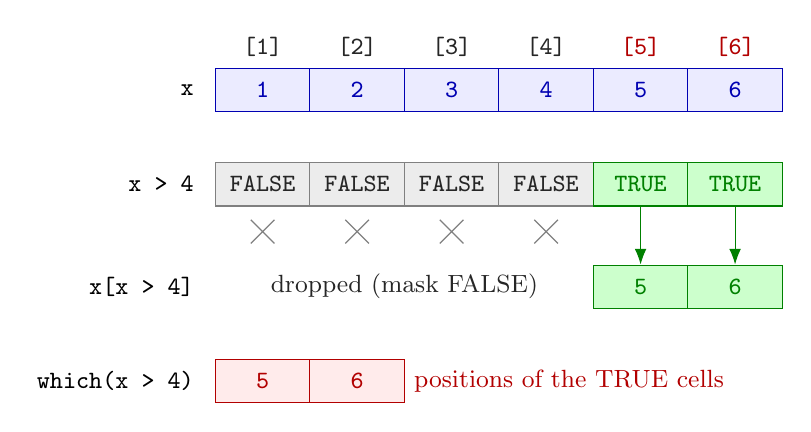
\begin{tikzpicture}[font=\small, >={Latex[length=2mm]},
  cell/.style={draw, minimum width=1.2cm, minimum height=0.55cm, inner sep=1pt, font=\small\ttfamily},
  val/.style={cell, draw=blue!70!black, fill=blue!8, text=blue!70!black},
  yes/.style={cell, draw=green!50!black, fill=green!20, text=green!50!black},
  no/.style={cell, draw=gray, fill=gray!15, text=gray!30!black},
  posn/.style={cell, draw=red!70!black, fill=red!8, text=red!70!black},
  lab/.style={anchor=east, font=\small\ttfamily},
  idx/.style={gray!30!black, font=\small\ttfamily}]
  \node[lab] at (0.45,0) {x};
  \foreach \v [count=\i] in {1,2,3,4,5,6} {
    \node[val] (a\i) at (1.2*\i,0) {\v};
  }
  \foreach \i in {1,2,3,4} { \node[idx] at (1.2*\i,0.55) {[\i]}; }
  \foreach \i in {5,6} { \node[red!70!black, font=\small\ttfamily] at (1.2*\i,0.55) {[\i]}; }
  \node[lab] at (0.45,-1.2) {x > 4};
  \foreach \s/\t [count=\i] in {no/FALSE,no/FALSE,no/FALSE,no/FALSE,yes/TRUE,yes/TRUE} {
    \node[\s] (b\i) at (1.2*\i,-1.2) {\t};
  }
  \foreach \i in {1,2,3,4} {
    \draw[gray, thin] (1.2*\i-0.15,-1.65) -- (1.2*\i+0.15,-1.95) (1.2*\i-0.15,-1.95) -- (1.2*\i+0.15,-1.65);
  }
  \node[lab] at (0.45,-2.5) {x[x > 4]};
  \foreach \i in {5,6} {
    \node[yes] (c\i) at (1.2*\i,-2.5) {\i};
    \draw[->, green!50!black] (b\i.south) -- (c\i.north);
  }
  \node[gray!30!black] at (3.0,-2.5) {dropped (mask FALSE)};
  \node[lab] at (0.45,-3.7) {which(x > 4)};
  \node[posn] at (1.2,-3.7) {5};
  \node[posn] at (2.4,-3.7) {6};
  \node[anchor=west, red!70!black] at (3.0,-3.7) {positions of the TRUE cells};
\end{tikzpicture}
\end{document}
